\subsection{The Autocorrelation Function Approach}
The generalized Langevin equation provides strategies for calculating position-dependent diffusion coefficients.  In these methods, the solute is restrained by a harmonic potential so that it oscillates at a point along the coordinate. The solute can now be described as a harmonic oscillator undergoing Langevin dynamics, where the balance of the system serves as the frictional bath for the solute. Implicitly, this requires the harmonic restraining potential to be dominant over the underlying free energy surface. 

The calculation of the friction coefficient from a harmonically-restrained MD simulation was originally used by Berne and coworkers in rate law calculations.\cite{BerneRateTheory1} Woolf and Roux elaborated this method to calculate position dependent diffusion coefficients.\cite{WoolfRouxDiffusion1994} In these approaches, the diffusion coefficient was calculated from the velocity autocorrelation function (VACF). This method requires the numerical Laplace transform of the VACF for several values of $s$ and extrapolation to the limit of $s=0$.

Hummer proposed a simplified method for calculating diffusion coefficients from a harmonicly restrained simulation.\cite{Hummer2005} In this method, the diffusion coefficient is be calculated directly from the integral of the autocorrelation function (ACF) of $z$ itself and the variance of $z$,

\begin{equation}
D(z= \langle z \rangle ) = \frac{\textrm{var}(z)^2}{\int_0^\infty \langle \delta z(0) \delta z(t) \rangle dt}
\label{eq:diff_hummer}
\end{equation}

This method is attractive because most molecular simulation codes can impose a harmonic restraint on a solute and save a time series of the $z$-position of this trajectory. The ACF can be calculated directly from the time series,\cite{Allen-Tildesley}
\begin{equation}
C_{zz}(t) =  \langle \delta z(0) \delta z(t) \rangle = \frac{1}{n_{samples}}\sum\limits_{i=0}^{n_{samples}} \delta z(i) \delta z(t+i)
\label{eq:correlation_sum}
\end{equation}
where $\delta z(t) = z(t)-z_0$. Correlation functions typically require extensive sampling to achieve convergence, particularly for long correlation times. Heterogeneity of the bilayer environment can cause the ACF calculated from different simulations at the same $z$-reference value to be significantly different. This can be addressed in part by performing several simulations, with a long equilibration period for each. The correlation functions can then be calculated from long time series collected from each of these simulations (e.g. $>$ 1 ns).

Although this method is a straightforward way to calculate membrane diffusion coefficient profiles, there are several practical issues associated with its use. We illustrate these issues by presenting the ACFs calculated from a simulation of urea restrained at 3 positions in the model bilayer system: $z=0$ \AA,  $z=10$ \AA, $z=36$ \AA. 

\begin{figure}
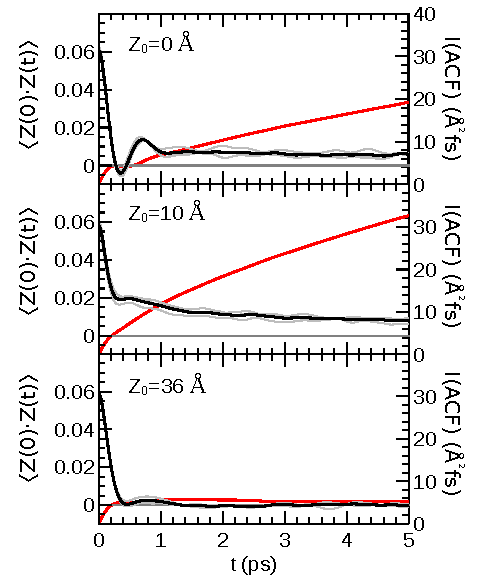
\includegraphics{acf-stacked}
\caption{The time autocorrelation function of urea in the model DMPC bilayer restrained at various values of $z_o$ using a harmonic potential ($U_{rest}=\frac{1}{2}k(z-z_o)^2)$). The black lines are the cumulative ACF calculated from three 1 ns simulations. The ACF from each 1 ns trajectory alone is presented in grey. The red lines (secondary axis) show the integral of the ACF in the interval $[0,t]$.}
\label{fig:acf}
\end{figure}

The general features of the ACFs can be interpreted based on the analytical solution autocorrelation function of a harmonic oscillator undergoing Langevin dynamics is a damped oscillating function,\cite{Tuckerman2010}
\begin{equation}
C_{zz}(t) = \textrm{var}(z) e^{-\gamma'(\bar \omega)t/2}[ \textrm{cos}(\Omega t) + \frac{\gamma'(\bar \omega)}{2 \Omega} \textrm{sin}(\Omega t)]
\label{eq:analytical-acf}
\end{equation}

The frictional coefficient of the Langevin damping ($\gamma'$) determines the rate of decay. There will be periodic oscillations in this function due to the sin/cos terms, but if the friction is high, the ACF may decay to zero before there are any significant oscillations. This is apparent in the ACF when the solute is restrained at  $z=36$ \AA\ (bulk water) (Figure \ref{fig:acf}), which decays to zero within 0.5 ps, but then has a short second peak extending to 1.2 ps.

The calculation of the diffusion coefficient formally requires the integration of ACF (\ref{eqn:hummer}) in the interval $[0, \infty]$, but the ACF will  decay to zero within $\sim$ 2 ps in most fluid environments. Even if extensive sampling has been performed, there can be significant noise on the ACF at long times. The g\_wham code avoids these issues by imposing a cutoff value.\cite{gwham} In that code, the integration is stopped when the ACF drops below a threshold value of $0.05 \times\ var(z)$. This is not appropriate in all instances because the ACF can go through multiple oscillations before converging to zero. Nevertheless, this strategy can provide reasonably accurate results if the autocorrelation function is dominated by a rapid decay  (i.e. in a high friction regime).

A second and more serious issue is apparent in the value of the autocorrelation functions in the lipid tail region at longer times (i.e. $>$ 2 ps). The simulations with $z_o=10$ \AA\ and $z_o=0$ \AA\ only decay to 8 and 13\% of their initial values in 5 ps. A consequence of the failure to converge to zero is that the integrated ACF increases linearly once the plateau is reached. These large values in the ACF at long times causes the calculated diffusion coefficients to be sensitive to the interval the ACF is integrated over. In general, this effect will cause the integrated autocorrelation to be larger than it should be, so the calculated diffusion coefficients are erroneously lowered due to this effect.

Although the bilayer interior is a lower-friction environment where one would expect the rate of decay to be slower, these ACFs do not converge to zero at long times due to other effects. Neale et al.\cite{Neale2011,Neale2014} showed that the convergence of in umbrella sampling simulations of solute permeation into bilayers can require 1 us length simulations. This due to very long correlation times in the values sampled in $z$-restrained umbrella sampling simulations and inhomogeneities in the bilayer interface that occur over very long time scales. While umbrella samplings simulations of the bilayer PMF can achieve convergence by running very long simulations, this lack of ergodicity in sampling is inconsistent with the underlying model of harmonic oscillator in frictional bath that is used to derive Eqn \ref{eqn:diff_hummer}.

These issues observed here are less serious for small solutes like water,\cite{Riahi2014,PeslherbeCholesterol} but they are severe for larger, more complex solutes like urea because they are more prone to have long-time correlations. In these cases, this method is not an appropriate way to calculate the diffusion coefficient profile. To determine if this issue is significant for a given system, the ACFs should be calculated and plotted for several $z$-positions in the bilayer. If the ACF has not decayed to values near 0 at long time scales (e.g. $>$ 2 ps), this method is probably not appropriate for calculating diffusion coefficient profiles for that solute.
